\documentclass{minimal}
\usepackage{epsfig,color}
\usepackage[papersize={400.00bp,200.00bp},text={400.00bp,200.00bp}]{geometry}
\begin{document}
\centering
% Title: glps_renderer figure
% Creator: GL2PS 1.3.8, (C) 1999-2012 C. Geuzaine
% For: Octave
% CreationDate: Mon Jun  1 17:07:52 2015
\setlength{\unitlength}{1pt}
\begin{picture}(0,0)
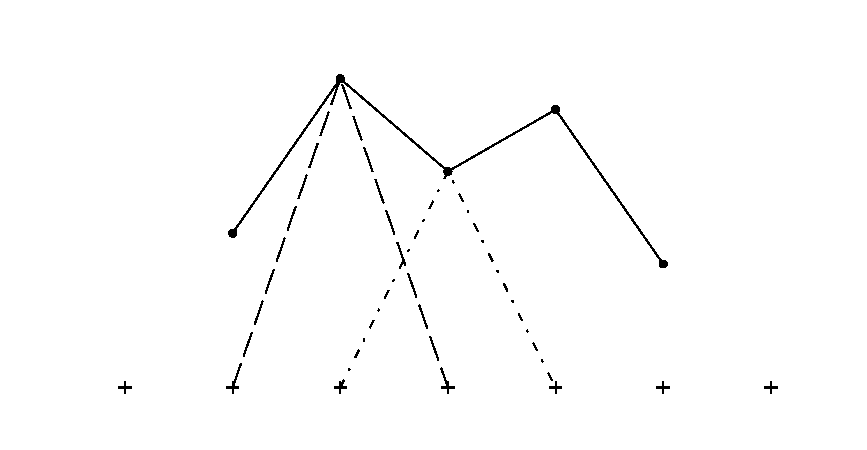
\includegraphics{linearBs-inc}
\end{picture}%
\begin{picture}(400,200)(0,0)
\fontsize{10}{0}
\selectfont\put(52,7.18182){\makebox(0,0)[tl]{\textcolor[rgb]{0,0,0}{${u_{i-2}}$}}}
\fontsize{10}{0}
\selectfont\put(103.667,7.18182){\makebox(0,0)[tl]{\textcolor[rgb]{0,0,0}{${u_{i-1}}$}}}
\fontsize{10}{0}
\selectfont\put(155.333,7.18182){\makebox(0,0)[tl]{\textcolor[rgb]{0,0,0}{${u_{i}}$}}}
\fontsize{10}{0}
\selectfont\put(207,7.18182){\makebox(0,0)[tl]{\textcolor[rgb]{0,0,0}{${u_{i+1}}$}}}
\fontsize{10}{0}
\selectfont\put(258.667,7.18182){\makebox(0,0)[tl]{\textcolor[rgb]{0,0,0}{${u_{i+2}}$}}}
\fontsize{10}{0}
\selectfont\put(310.333,7.18182){\makebox(0,0)[tl]{\textcolor[rgb]{0,0,0}{${u_{i+3}}$}}}
\fontsize{10}{0}
\selectfont\put(362,7.18182){\makebox(0,0)[tl]{\textcolor[rgb]{0,0,0}{${u_{i+4}}$}}}
\fontsize{10}{0}
\selectfont\put(88.1667,110.909){\makebox(0,0)[tl]{\textcolor[rgb]{0,0,0}{${x_{i-2}}$}}}
\fontsize{10}{0}
\selectfont\put(150.167,185){\makebox(0,0)[tl]{\textcolor[rgb]{0,0,0}{${x_{i-1}}$}}}
\fontsize{10}{0}
\selectfont\put(207,140.545){\makebox(0,0)[tl]{\textcolor[rgb]{0,0,0}{${x_{i}}$}}}
\fontsize{10}{0}
\selectfont\put(253.5,170.182){\makebox(0,0)[tl]{\textcolor[rgb]{0,0,0}{${x_{i+1}}$}}}
\fontsize{10}{0}
\selectfont\put(310.333,96.0909){\makebox(0,0)[tl]{\textcolor[rgb]{0,0,0}{${x_{i+2}}$}}}
\end{picture}
\end{document}
